% This is samplepaper.tex, a sample chapter demonstrating the
% LLNCS macro package for Springer Computer Science proceedings;
% Version 2.20 of 2017/10/04
%
\documentclass[runningheads]{llncs}
%
\usepackage{graphicx,wrapfig,xcolor,subfig}
\usepackage{amstext,amsmath,amssymb,bm,bbm,mathtools}
\usepackage{array,multirow}
\usepackage{algorithm2e}

\newcommand{\daniel}[1]{ {\color{black}#1} }

\DeclarePairedDelimiter\norm{\lVert}{\rVert}%
\DeclareMathOperator*{\argmin}{arg\,min}

%% Daniel's definitions
\newcommand{\Ds}{D}
\newcommand{\GG}{ \mathcal{G}_{\vec{I}} }
\newcommand{\GGe}{ \mathcal{G}_{\vec{I}+} }
\newcommand{\GGc}[1]{ \mathcal{G}_C^{(#1)} }
\newcommand{\GGcc}{ \mathcal{G}_C}

\newcommand\figTable[2]{\raisebox{-.5\height}{\includegraphics[scale=#1]{#2}}}

\newcommand\segComparisonGF[2]{figures/segmentation/comparison/#1/#2/alpha-0.0002/beta-1.0/gamma-3.0/radius-7}
\newcommand\segComparisonFF[2]{figures/segmentation/comparison/#1/#2/alpha-0.5/beta-1.0/gamma-3.0/radius-7}
\newcommand\segComparisonScho[2]{figures/segmentation/comparison/#1/lambda-2.0/gamma-1.0/#2}

\begin{document}
%
\title{A maximum-flow model for digital elastica shape optimization}
%
%\titlerunning{Abbreviated paper title}
% If the paper title is too long for the running head, you can set
% an abbreviated paper title here
%
\author{Daniel Martins Antunes\inst{1}\orcidID{0000-0002-6752-0217} \and
Jacques-Olivier Lachaud\inst{1}\orcidID{0000-0003-4236-2133} \and
Hugues Talbot\inst{2}\orcidID{0000-0002-2179-3498}}
%
\authorrunning{D. Martins Antunes et al.}
% First names are abbreviated in the running head.
% If there are more than two authors, 'et al.' is used.
%
\institute{Universit\'e Savoie Mont-Blanc, France
\email{\{daniel.martins-antunes,jacques-olivier.lachaud\}@univ-smb.fr}\\
\and
CentraleSupelec, Universit\'e Paris-Saclay, Inria\\
\email{\{hugues.talbot\}@centralesupelec.fr}}
%
\maketitle              % typeset the header of the contribution
%
\begin{abstract}
  The Elastica is a curve regularization model that integrates the squared curvature in addition to the curve length. It
  has been shown to be useful for contour smoothing and interpolation, for example in the presence of thin
  elements.

  In this article, we propose a graph-cut based model for optimizing the discrete Elastica energy using a fast and
  efficient graph-cut model.  Even though the Elastica energy is neither convex nor sub-modular, we show that the final
  shape we achieve is often very close to the globally optimal one.

  Our model easily adapts to image segmentation tasks. We show that compared to previous works and state-of-the-art
  algorithms, our proposal is simpler to implement, faster, and yields comparable or better results.

  \keywords{multigrid  convergence \and digital estimators \and curvature \and discrete optimization}
\end{abstract}
%
%
%
\section{Introduction}

The Elastica model and associated energy is a curve regularisation problem with a rich
history~\cite{matsutani2010euler,levien08elastica}, which involves the squared curvature.  It was introduced in computer
vision in~\cite{mumford94elastica} as a means to regularize edges or segmentation boundaries with an explicit curvature
component. Being associated with second-order derivatives, the notion of curvature is difficult to compute and optimize
in a regularisation framework.

Multiple attempts have been made by prominent researchers to introduce
an explicit curvature term in curve regularizers using various methods
and approaches. Even early active contour models~\cite{kass88} had an
elasticity component equivalent to a notion of curvature. Similarly,
with level-set methods, local curvature can readily be estimated as
in~\cite{malladi1995shape}. However these approaches typically
optimise a non-convex local energy by gradient descent, and most were
non-geometric, i.e discretization-dependent. In
contrast~\cite{caselles97} proposed a geometric level-set segmentation
method, but using only the perimeter as a regularizer, and was still
non-convex. All the numerous approaches based on total-variation
minimization for image restoration or
segmentation~\cite{rudin1992nonlinear} and even the Mumford-Shah
functional~\cite{mumford89} use this quite elementary regularizer,
probably because optimizing it in an exact manner was already a
challenge for a long
time~\cite{boykov01fast,chambolle04,appleton2005globally}, whether in
the discrete or continuous cases.

In more recent works, optimizing the Elastica, which is a geometric regularizer, has seen renewed
interest. In~\cite{masnou98inpainting}, authors successfully use a computational geometry approach to perform image
restoration with the Elastica as regularizer. In~\cite{zehiry10fast}, authors compute an approximate discrete version of
the Elastica and optimize it with discrete calculus. In~\cite{nieuwenhuis14efficient}, an efficient, discrete
approximation of curvature is optimized with a specific solver using local submodular
approximations~\cite{gorelick14local}. However, in these works, the poor quality of the curvature approximation may limit accuracy and hence the quality of the result.

In a previous work~\cite{antunes2020elastica} we proposed to formulate a digital flow that approximates an
Elastica-related flow using a multigrid-convergent curvature estimator, within a discrete variational
framework. We also presented an application of this model as a post-processing step to a segmentation framework.

In this work, we propose a novel approach that still uses a
multigrid-convergent estimation of curvature, but we optimize using a
maximal flow algorithm.

\subsection{Multigrid convergent estimators}
Geometric measurements in digital objects can be tricky.  Intuitively, a good estimator should converge to its
continuous counterpart value as the grid resolution is refined. The criterion that formalizes this intuition is the
multigrid convergence property.

\begin{definition}{(Multigrid convergence)}
  Let $\mathcal{F}$ a family of shapes in the plane and $Q$ a global measurement (e.g., perimeter, area) on members of
  $\mathcal{F}$. Additionally, denote $D_h(S)$ a digitization of shape $S$ in a digital grid of resolution $h$. The
  estimator $\hat{Q}$ of $Q$ is {\em multigrid convergent} for the family $\mathcal{F}$ if and only if for every shape
  $S \in \mathcal{F}$, there exists $h_S > 0$ such that
\begin{align*}
\forall h \leq h_S, \quad |\hat{Q}(D_h(S),h) - Q(S)| \leq \tau_S(h),
\end{align*}
%
where $\tau_S:\mathbb{R}_+\setminus \{0\} \rightarrow \mathbb{R}_+$ tends to zero as $h$ tends to zero and is the {\em speed of convergence} of $\hat{Q}$ towards $Q$
for $S$.
\end{definition}

Tangent and curvature are examples of local properties computed along the boundary of some shape $S$ in the plane. We
need a slightly different definition of multigrid convergence in order to map points of the Euclidean boundary to those in
the digital contour.

\begin{definition}{(Multigrid convergence for local geometric quantities)}
  Let $\mathcal{F}$ a family of shapes in the plane and $Q$ a local measurement along the boundary $\partial S$ of
  $S \in \mathcal{F}$. Additionally, denote $D_h(S)$ a digitization of $S$ in a digital grid of resolution $h$ and
  $\partial_h S$ its digital contour. The estimator $\hat{Q}$ of $Q$ is {\em multigrid convergent} for the family
  $\mathcal{F}$ if and only if for every shape $S \in \mathcal{F}$, there exists $h_S > 0$ such that the estimate
  $\hat{Q}(D_h(S),p,h)$ is defined for all $p \in \partial_h S$ with $0 < h < h_S$, and for any $x \in \partial S$,
\begin{align*}
	\forall p \in \partial_h S \text{ with } \norm{p-x}_{\infty} \leq h,\quad | \hat{Q}(D_h(S),p,h) - Q(S,x) | \leq \tau_S(h),	
\end{align*}
where $\tau_S:\mathbb{R}_+\setminus \{0\} \rightarrow \mathbb{R}_+$ has null limit at $0$. This function defines the
{\em speed of convergence} of $\hat{Q}$ towards $Q$ for $S$.
\end{definition}

We now recall the notion of Elastica, as well as its digital counterpart.

\subsection{Digital Elastica}
Letting $\kappa$ be the curvature function along some Euclidean shape
$S \subset \mathbb{R}^2$. The elastica energy of $S$ with parameters
$\vec{\theta}=(\alpha \geq 0, \beta \geq 0)$ is defined as
	\begin{align*}
	E_{\vec{\theta}}(S) &= \int_{\partial S}{ \alpha + \beta \kappa(s)^2 ds}.
	\end{align*}
Similarly, the digital elastica $\hat{E}_{\vec{\theta}}$ of some digitization $D_h(S)$ of $S$ is defined as
	\begin{align}
	\hat{E}_{\vec{\theta}}( D_h(S) ) = \sum_{\dot{\vec{e}} \in \partial_h S}{ \hat{s}( \dot{\vec{e}})\left(\; \alpha + \beta \hat{\kappa}^2(D_h(S),\dot{\vec{e}},h) \; \right)},
	\label{ch5:digital-elastica}
	\end{align}
where $\dot{\vec{e}}$ denotes the center of the linel $\vec{e}$ and the estimators of length $\hat{s}$ and
curvature $\hat{\kappa}$ are multigrid convergent.


\subsection{A multigrid-convergent estimation of curvature}    
Let $S$ be an arbitrary shape. The following definition yields a curvature estimation at every point of its boundary.

\begin{definition}{(Integral Invariant Curvature Estimator)}
  Let $D_h(S)$ a digitization of $S \subset \mathbb{R}^2$ \daniel{and $B_r(p)$ the Euclidean disk of radius $r$ centered at $p$}. The integral invariant curvature estimator is defined for
  every point $p \in \partial_h S$ as
  \begin{align}
    \hat{\kappa}_{r}(D_h(S),p,h) \coloneqq \frac{3}{r^3} \left( \frac{\pi r^2}{2} - \widehat{\text{Area}} \left( D_h\big( B_{r} ( p ) \big) \cap D_h(S), h \right) \right).
    %% \hat{\kappa}_{r}(D,x,h) \coloneqq \frac{3}{r^3} \left( \frac{\pi r^2}{2} - \widehat{Area} \left( B_{r/h} ( \frac{1}{h} \cdot x ) \cap D, h \right) \right),
    \label{eq:curvature_approximation}
  \end{align}
\end{definition}
%
where $\widehat{\text{Area}}( D,h )$ estimates the area of $D$ by counting its grid points and then scaling them by
$h^2$. This estimator is multigrid convergent for the family of compact shapes in the plane with $3$-smooth boundary. It
converges with speed $O(h^\frac{1}{3})$ for radii chosen as $r=\Theta(h^\frac{1}{3})$~\cite{lachaud17robust}.

In the expression above, we will substitute an arbitrary
subset $\Ds$ of $\mathbb{Z}^2$ to $D_h(S)$ since the continuous shape $S$ is unknown.  In the following we omit
the grid step $h$ to simplify expressions (or, putting it differently, we assume that the shape of interest is
rescaled by $1/h$ and we set $h=1$).


\section{Digital elastica minimization via graph cuts}
In this section we present a graph cut model that converges to the optimum digital shape under digital elastica
regularization. Moreover, the model is easily adapted to image segmentation tasks. 

\daniel{\subsection{Balance Coefficient}
In the core of the model is the notion of balance coefficient. We are going to extend equation~\ref{eq:curvature_approximation} to the whole digital domain. In fact, since we are more interested in the  balance of intersected and non-intersected points, we slightly change equation~\ref{eq:curvature_approximation} and give it another name. We define the \emph{balance coefficient} as
%
\begin{align*}
%% JACO: attention j'ai change D en dessous.
  u_r(D,p) &= \left( \frac{\pi r^2}{2} - \widehat{\text{Area}}(B_r(p) \cap D) \right)^2.
	%% u_r(D,p) &= \left( \frac{\pi r^2}{2} - \widehat{\text{Area}}(D(B_r(p)) \cap D) \right)^2.
\end{align*}
%
 The balance coefficient at $p$ gives us as an \emph{approximation} of the new squared curvature value when the shape is perturbed a little around $p$. Therefore, it is reasonable to evolve the shape towards the zero level set of the balance coefficient function (see figure~\ref{fig:balance-coefficient-zero-level-set}).
 %
\begin{figure}
 \center
 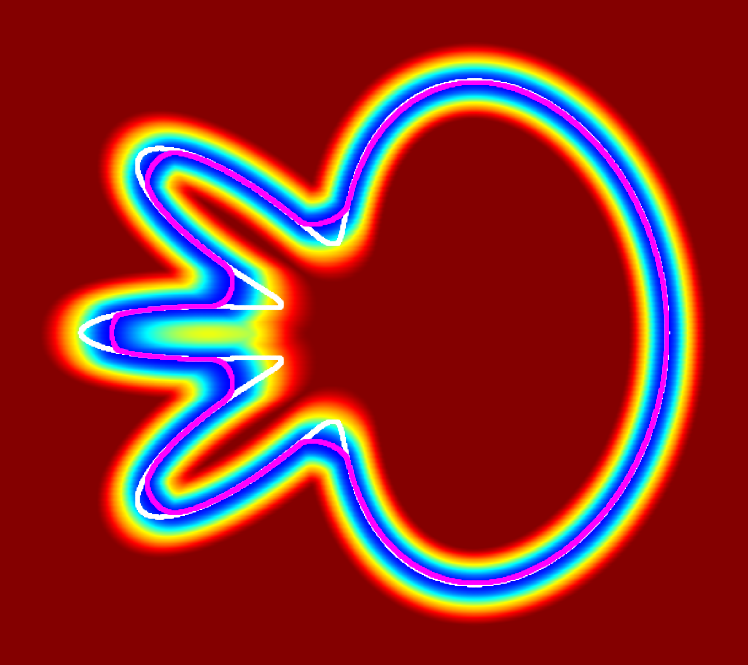
\includegraphics[scale=0.32]{figures/zero-level-set/balance-coefficient-zero-level-set.png}
 \caption{\textbf{Balance coefficient zero level set}. We notice that evolving the initial contour (colored in white) to the zero level set of the balance coefficient (colored in magenta) regularizes the shape with respect to the squared curvature.}
 \label{fig:balance-coefficient-zero-level-set}
 \end{figure}}
%

\subsection{Model overview}
Let $D^{(0)}$ be the initial digital set. The GraphFlow model produces a sequence of digital shapes $D^{(k)}$ by executing two main steps:
%
\begin{itemize}
\item[]{\textbf{Candidate selection:} We associate to $D^{(k)}$ a set of neighbor shapes $\mathcal{P}(D^{(k)})$. For
    each $D' \in \mathcal{P}(D^{(k)})$ we construct the capacitated graph $\mathcal{G}_{D'}$ such that its minimum cut $Q$ minimizes the candidate function.
\begin{align}
	cand(D) &= data(D) + \sum_{p \in D'}\sum_{q \in \mathcal{N}_{4}(p)}{ u_r(D,p) +u_r(D,q) }. \label{eq:candidate-function}
\end{align}
The proposition $mincut(Q,G)$ indicates that $Q$ is a minimum cut of $G$.}
\vspace{1em}
\item[]{\textbf{Validation:} Each minimum cut $Q$ computed in the previous step induces a solution candidate $D_{Q}$. We group the solution candidates in the set $sol(D^{(k)})$ and we choose the one that minimizes the validation energy
\begin{align}
	val(D) &= data(D) + \hat{E}_{\vec{\theta}}( D ). \label{eq:validation-function}
\end{align}
}
\end{itemize}
%
The candidate function is computed on a band around the contour of $D^{(k)}$. Let $d_{D}:\Omega \rightarrow \mathbb{R}$ be the signed Euclidean distance transformation with respect to shape $D$. The value $d_{D}(p)$ gives the Euclidean distance between $p \notin D$ and the closest point in $D$. For points $p \in D$, $d_{D}(p)$ gives the negative of the distance between $p$ and the closest point not in $D$.
%
\begin{definition}{(Optimization band)}
Let $D \subset \Omega \subset \mathbb{Z}^2$ a digital set and natural number $n>0$. The optimization band $O_n(D)$ is defined as
\begin{align*}
	O_n(D) &:=\left\{ p \in \Omega \; | \; -n \leq d_{D}(p) \leq n \right\}.
\end{align*}
\end{definition}
%
We use as the neighborhood of shapes the $a$-probe set
%
\begin{definition}{($a$-probe set)}
	Let $\Ds \subset \Omega \subset \mathbb{Z}^2$ a digital set and $a$ some natural number. The $a$-probe set of $\Ds$ is defined as
	\begin{align*}
		\mathcal{P}_a(\Ds) &= \Ds \cup \bigcup_{a' < a}{\Ds^{+a'} \cup \Ds^{-a'}},
	\end{align*}
	where $\Ds^{+a}$($\Ds^{-a}$) denotes a dilation(erosion) by a disk of radius $a$.
\end{definition}
%

\daniel{
\subsection{Shape optimization}
We are going to evolve the initial contour $\partial D$ of some digital shape $D$ to the zero level set of its balance coeficient by computing the minimum cut of the candidate graphs. In this experiment, the data term in both candidate and validation functions equal to zero.}
%
\begin{definition}{Candidate graph}
Let $D \subset \Omega \subset \mathbb{Z}^2$ a digital set and natural number $n>0$. We define $\mathcal{G}_D(\mathcal{V},\mathcal{E},c)$ as the candidate graph of $D$ with optimization band $n$ such that
%
\begin{align*}
\mathcal{V} &= \big\{\; v_p \; | \; p \in O_n(D) \;\} \cup \{s,t \big\} \\
\mathcal{E} &= \big\{ \; \{v_p,v_q\} \; | \; p \in O_n(D) \text{ and } q \in \mathcal{N}_4(p) \; \big\} \cup \mathcal{E}_{st}\\
\mathcal{E}_{st} &= \big\{\; \{s,v_p\} \; | \; d_D(p)=-n \; \big\} \cup \big\{\; \{v_p,t\} \; | \; d_D(p)=n \; \big\}.
\end{align*}
%
\end{definition}

The vertices $s,t$ are virtual vertices representing the source and target vertices as it is usual in a minimum cut framework. In particular, after the minimum cut is computed, vertices connected to the source will define the new digital shape. The innermost (resp. outermost) pixels of the optimization band are connected to the source (resp. target), and we identify such vertices as
%
\begin{align*}
	\mathcal{V}_s &:=\left\{ v_p \in \Omega \; | \; d_{D}(p) = -n \right\} \\
	\mathcal{V}_t &:=\left\{ v_p \in \Omega \; | \; d_{D}(p) = n \right\}.
\end{align*}
%
The set $\mathcal{E}_{st}$ comprises all the edges having the source as their starting point or the target as their endpoint. Next, we describe how to set the edges' capacities.

\begin{center}
\begin{tabular}{|c|c|c|}
\hline
\textbf{edge} $e$ & $\mathbf{c(e)}$ & \textbf{for}\\
\hline
$\{v_p, v_q\}$ & $ u_r(D,p) + u_r(D,q) $ & $\{v_p,v_q\} \in \mathcal{E}_{u}$\\
\hline
$\{v_p, s\}$ & $M$ & $v_p \in \mathcal{V}_{s}$ \\
\hline
$\{v_p, t\}$ & $M$ & $v_p \in \mathcal{V}_{t}$ \\
\hline
\end{tabular}
\end{center}


Here $M$ is twice the highest value of the balance coefficient plus one, i.e.
\begin{align*}
	M &= 1+\max_{p \in O_n(D)} 2*u_r(D,p).
\end{align*}
%

\daniel{\subsection{Image segmentation}
The GraphFlow model is suitable for image processing tasks. We present our experiments using the data term employed by Boykov-Jolly (BJ) graph cut model described in~\cite{boykov01graphcut}. Let $\vec{x} \in [0,1]^{|D|}$ represent the label of each pixel ($0$ for background and $1$ for foreground). Then, we define the data term as
%
\begin{align*}
	data(D) &= \gamma_r \sum_{p \in D}{ \psi_p(x_p) } + \gamma_b \sum_{p \in D'}\sum_{q \in \mathcal{N}_{4}(p)}{\psi_{p,q}(x_p,x_q)},
\end{align*}
where $\gamma_r \geq 0$ and $\gamma_b \geq 0$ are parameters controlling the influence of the data and space coherence terms, respectively. Given the image $I:\Omega \rightarrow [0,1]^3$, the unary and pairwise terms are defined as}
\begin{align*}
	\psi_p(x_p) &= \left\{ \begin{array}{ll}
	-\ln  H_{bg}\big( I(p) \big), & \text{if } x_p=0  \\[1em]	
	-\ln  H_{fg}\big( I(p) \big), & \text{if } x_p=1,
	\end{array}\right.\\[1em]
	\psi_{p,q}(x_p,x_q) &= \left\{ \begin{array}{ll}
	\displaystyle \exp{ \left(- \frac{1}{ |(p,q)| }\frac{(I(p) - I(q))^2}{2\sigma^2} \right) }, & q \in \mathcal{N}_4(p) \\[1em]
	0, & \text{otherwise}.
	\end{array}\right.
\end{align*}
%
\daniel{The terms $H_{bg}$ and $H_{fg}$ are mixed Gaussian distribution constructed from foreground and background seeds given by the user. }
%Therefore, the GraphFlow model can be seen as an extension of the BJ graph cut segmentation model with a regularization term based on squared curvature. However, the GraphFlow model needs an initial solution, which is given by the BJ model (no curvature regularization).
%
%
\subsection{Elastica GraphFlow algorithm}
The GraphFlow algorithm implements a local-search strategy to minimize~\eqref{eq:validation-function} with a search
space given by the solution of the candidates set defined in the previous section. We choose to let the model flow even in the case
where the next shape $D^{(k+1)}$ has a higher energy than the previous shape $D^{(k)}$. It is a simple strategy to escape local minima. In the implementation
presented here, the only stopping condition is the number of iterations. This strategy could be tailored to a specific application.

%
\begin{algorithm}
 \SetKwData{It}{k}
 \SetKwData{MIt}{maxIt}
 \SetKwData{Delta}{delta}
 \SetKwInOut{Input}{input}\SetKwInOut{Output}{output}
 \SetKwComment{comment}{//}{}
 
 \Input{An image $I$ or a digital set $D$; the optimization band $n$; the probe set parameter $a$; parameter vector $\vec{\theta}=(\alpha,\beta)$; parameter vector $\vec{\gamma} = (\gamma_r,\gamma_b)$; the maximum number of iterations \MIt;} 
 \BlankLine
 \If{ Image $I$ is given }
 {
	 $\Ds^{(0)} \longleftarrow graphcut_BJ(I)$\;  
 }
 \Else{
	 $\Ds^{(0)} \longleftarrow \Ds$\; 
	 $(\gamma_r,\gamma_b) \longleftarrow (0,0)$\; 	 
 }
 \BlankLine
 $k \longleftarrow 0$\;
 \While{ \It $<$ \MIt  }{ 	
	\comment{Candidate selection} 
	$sol(D^{(k)}) \longleftarrow \bigcup_{D' \in \mathcal{P}_a(D^{(k)})} \Big\{ \big( Q,D_Q \big) \; | \; mincut(Q,\mathcal{G}_{D'}) \Big\}$ \;

	\BlankLine
	\comment{Candidate validation}
	$\Ds^{(k+1)} \longleftarrow \displaystyle \argmin_{ (Q,S) \in sol(D^{(k)}) }{ data(S) + \hat{E}_{\vec{\theta}}(S) }$\; 	
	\It $\longleftarrow$ \It $+1$\;
	
 }
 \caption{GraphFlow algorithm.}
 \label{ch8:alg:graphflow-algorithm}  
\end{algorithm}
%
The Elastica GraphFlow algorithm has two fundamental steps. In the candidate selection, we build the solution of the candidates
set from the minimum cuts of the candidate graphs. Next, in the validation step, we choose the digital set with minimum
value for~\eqref{eq:validation-function}. If we interpret the balance coefficient minimization as the best move one can
make towards digital elastica minimization, the solution of the candidates set can be seen as the neighboring shapes with
highest potential to minimize the elastica energy for the given $a$-probe set.

Some results of Algorithm~\ref{ch8:alg:graphflow-algorithm} are shown in the next section.

\section{Results and discussion}
We first present some of our own results, then some comparison with our previous work and with the reference
implementation of~\cite{schoenemann09linear}.

\subsection{Results}
The GraphFlow algorithm produces a flow that is in accordance with expectations for a flow guided by the elastica
energy. In particular, it grows and shrinks in accordance with the $\alpha$ coefficient in the digital elastica
(see Fig.~\ref{ch8:fig:graph-flow-neigh2-results}) \daniel{for $a$-probe sets such that $a>0$}. \daniel{If we use a $0$-probe set, we recover a flow similar to the curve-shortening flow~\cite{huisken84flow}.}
\begin{figure}
\center
\subfloat[]{
\begin{tabular}{ccc}

\includegraphics[scale=0.20]{figures/triangle/neigh-0/alpha-0.01/summary.pdf} & 
\includegraphics[scale=0.20]{figures/triangle/neigh-2/alpha-0.01/summary.pdf} & 
\includegraphics[scale=0.20]{figures/triangle/neigh-2/alpha-0.001/summary.pdf}\\
$(n=2, a=0,\alpha=0.01)$ & $(n=2, a=2,\alpha=0.01)$ & $(n=2, a=2, \alpha=0.001)$
\end{tabular}}
\caption{\textbf{GraphFlow results.} The GraphFlow algorithm can shrink and grow in accordance with length penalization
  and it converges to a shape close to the theoretical global optimum (green curve) in the free elastica problem. We are using $n=2,a=2$ and shapes are displayed every $10$ iterations.\label{ch8:fig:graph-flow-neigh2-results}}
\end{figure}
%
%
\begin{figure}
\center
\begin{tabular}{cccc}
\multirow{2}{*}{Seeds} & \multirow{2}{*}{Graph cut} & $\alpha=0.05, \boldsymbol{\beta=0},$ & $\alpha=0.05, \boldsymbol{\beta=0.5},$\\
& & $\gamma_r=\gamma_b=1.0$ & $\gamma_r=\gamma_b=1.0$\\
 	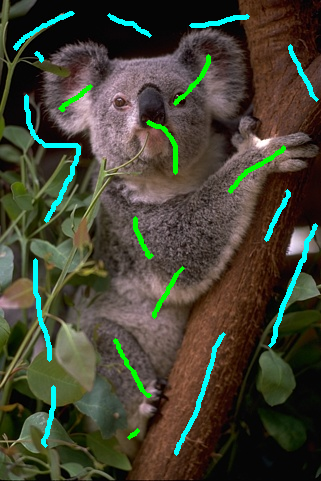
\includegraphics[scale=0.25]{figures/segmentation/coala/k-00-seeds.png} & 
 	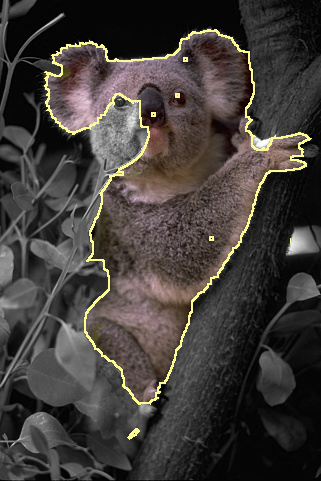
\includegraphics[scale=0.25]{figures/segmentation/coala/k-00-gc-seg.png} &  	
 	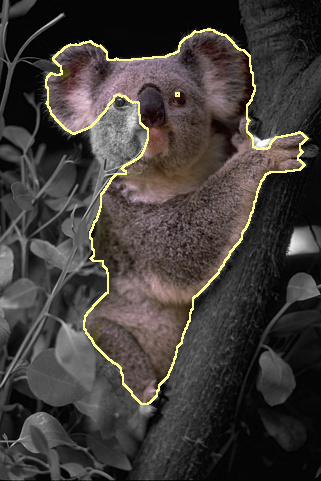
\includegraphics[scale=0.25]{figures/segmentation/coala/k-00-corrected-seg.png} &  	
 	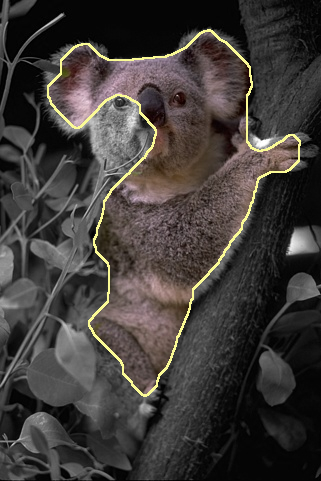
\includegraphics[scale=0.25]{figures/segmentation/coala/k-05-corrected-seg.png}
\end{tabular}	
\caption{\textbf{GraphFlow segmentation.} Given foreground (green) and background (gray) seeds in picture (a); Graph cut
  produces picture (b) which is used as input of the GraphFlow algorithm; in pictures (c) and (d) we display the output
  of our Elastica GraphFlow algorithm with and without the squared curvature term in the regularization. }
\label{ch8:fig:segmentation}
\end{figure}
%
\begin{figure}
\center
\begin{tabular}{cc}
$\alpha=0, \boldsymbol{\beta=0}$ & $\alpha=0, \boldsymbol{\beta=1}$\\
$\gamma_r = 3, \gamma_b = 3$ & $\gamma_r = 3, \gamma_b = 3$\\
 	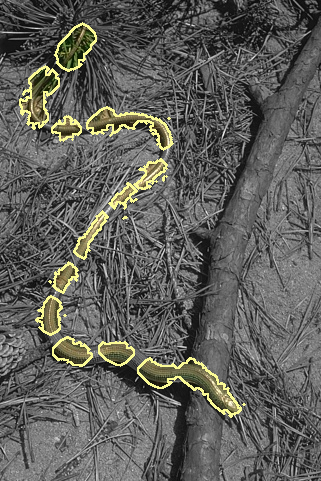
\includegraphics[scale=0.35]{figures/completion/graphseg/alpha-0.0/beta-0.0/gamma-3.0/radius-7/corrected-seg.png} & 
 	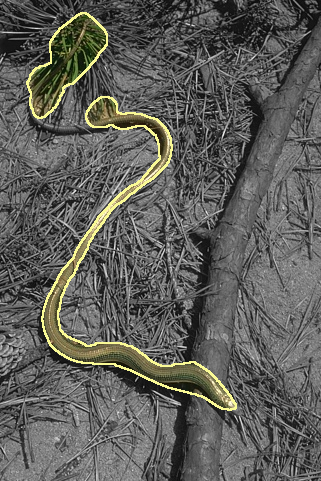
\includegraphics[scale=0.35]{figures/completion/graphseg/alpha-0.0/beta-1.0/gamma-3.0/radius-7/corrected-seg.png}
\end{tabular}	
\caption{\textbf{GraphFlow and completion property}. The oversegmented picture on the left was obtained with no squared curvature regularization, while the picture on the right was obtained by setting $\beta=1.0$. }
\label{ch8:fig:segmentation-curvature-completion}
\end{figure}
%
The solutions are very similar to those achieved in~\cite{antunes2020elastica}, but with the advantage of producing
smoother flows and up to $100 \times$ faster.  In Fig.~\ref{ch8:fig:segmentation}, we show that our algorithm can easily
be used for segmentation, and that it produces results that are parametrically smoother than those of the BJ model.

In Fig.~\ref{ch8:fig:segmentation-curvature-completion}, we can observe that the Elastica GraphFlow presents the completion
property, i.e., it tends to return a segmentation with fewer disconnected components.

\subsection{Comparisons}
In this section we compare our proposed results for segmentation with several state-of-the-art results in
Fig~\ref{ch9:fig:exp-comparison-image-segmentation-1}: the reference BJ segmentation method; the linear relaxation
methods by Schoeneman \emph{et al.}; and our previous results.
%
\begin{figure}
	\centering
	\setlength{\tabcolsep}{1pt}
	\begin{tabular}{m{0.25cm}ccc}
          \rotatebox{90}{Graph cut~\cite{boykov01graphcut}} & 
	\figTable{0.25}{\segComparisonFF{flipseg}{airplane}/gc-seg.png} & 
	\figTable{0.25}{\segComparisonFF{flipseg}{kite-surf}/gc-seg.png} & 
	\figTable{0.25}{\segComparisonFF{flipseg}{mans-music}/gc-seg.png} \\[6em]
	
	\rotatebox{90}{SCLR~\cite{schoenemann09linear}} & 
	\figTable{0.25}{\segComparisonScho{schoenemann}{airplane}/airplane.png} & 
	\figTable{0.25}{\segComparisonScho{schoenemann}{kite-surf}/kite-surf.png} & 
	\figTable{0.25}{\segComparisonScho{schoenemann}{mans-music}/mans-music.png}\\[6em]
	
	\rotatebox{90}{Previous work~\cite{antunes2020elastica}} & 
	\figTable{0.25}{\segComparisonFF{flipseg}{airplane}/corrected-seg.png} & 
	\figTable{0.25}{\segComparisonFF{flipseg}{kite-surf}/corrected-seg.png} & 
	\figTable{0.25}{\segComparisonFF{flipseg}{mans-music}/corrected-seg.png} \\[6em]
		
	\rotatebox{90}{GraphFlow (proposed)} & 
	\figTable{0.25}{\segComparisonGF{graphseg}{airplane}/corrected-seg.png} & 
	\figTable{0.25}{\segComparisonGF{graphseg}{kite-surf}/corrected-seg.png} & 
	\figTable{0.25}{\segComparisonGF{graphseg}{mans-music}/corrected-seg.png}
	\end{tabular}
	\caption{\textbf{Segmentation results comparison. Top row, Graph-Cut BJ results; second row: references SCLR
            results; third row: previous results from~\cite{antunes2020elastica}; last row: proposed method. }}
	\label{ch9:fig:exp-comparison-image-segmentation-1}
      \end{figure}
%
 We observe that our results are smoother than BJ, as in the previous figure. They are very similar to our previous
 results, and much better than the reference SCLR method from literature.

\begin{table}[t]
  \centering
 \caption{Running time for the image segmentation problem.}
\label{ch9:tab:rtime-image-segmentation-general} 
\captionsetup{type=table}
\begin{tabular}{|c|c|c|c|}
\hline
\multicolumn{4}{|c|}{Exp-Comparison Running time}\\
\hline
Model & Minimum & Maximum & Average \\
\hline
SLCR & 2.87min & 52.24min & 18.4min\\
Previous work & 60s & 297s & 156s\\
This work  & 11s & 150s & 75s\\
\hline
\end{tabular}
\end{table}

\daniel{All the experiments were executed on a 32-core 2.4Ghz CPU}. According to Table~\ref{ch9:tab:rtime-image-segmentation-general}, our proposed method is signifiantly faster than
our previous work, and much faster than the reference SLCR method.

\section{Conclusion}
In this article, we described a graph cut model for optimizing the
Elastica energy that is suitable for both discrete curve evolution and
image segmentation. The evolution produced by the Elastica GraphFlow
responds to the length penalization term $\alpha$, i.e., the shape
tends to grow (shrink) for lower (higher) values of $\alpha$ and to
the curvature penalization $\beta$. Furthermore we observe a
convergence to a shape that appears close to the expected, theoretical
global optimum of the Elastica model in the cases where this globally
optimal curve can be computed. Our Elastica GraphFlow algorithm is
significantly faster and simpler to implement than the previous models
presented in the literature.

In our method, we need to use a family of shapes ($a$-probes). In future work, we plan to use a dynamic family with the
help a parameter-free estimator. In the same vein, a multi-resolution approach would be very useful, in particular for
dealing with very thin portions of the image. We also note that a globally optimal solution with multigrid convergent
estimators is yet to be proposed. 

\bibliographystyle{splncs04}
\bibliography{discrete_elastica_dgmm_2021}

\end{document}



%%% the rest below is for reference

\subsubsection{Sample Heading (Third Level)} Only two levels of
headings should be numbered. Lower level headings remain unnumbered;
they are formatted as run-in headings.

\paragraph{Sample Heading (Fourth Level)}
The contribution should contain no more than four levels of
headings. Table~\ref{tab1} gives a summary of all heading levels.

\begin{table}
\caption{Table captions should be placed above the
tables.}\label{tab1}
\begin{tabular}{|l|l|l|}
\hline
Heading level &  Example & Font size and style\\
\hline
Title (centered) &  {\Large\bfseries Lecture Notes} & 14 point, bold\\
1st-level heading &  {\large\bfseries 1 Introduction} & 12 point, bold\\
2nd-level heading & {\bfseries 2.1 Printing Area} & 10 point, bold\\
3rd-level heading & {\bfseries Run-in Heading in Bold.} Text follows & 10 point, bold\\
4th-level heading & {\itshape Lowest Level Heading.} Text follows & 10 point, italic\\
\hline
\end{tabular}
\end{table}


\noindent Displayed equations are centered and set on a separate
line.
\begin{equation}
x + y = z
\end{equation}
Please try to avoid rasterized images for line-art diagrams and
schemas. Whenever possible, use vector graphics instead (see
Fig.~\ref{fig1}).
%
\begin{figure}
\includegraphics[width=\textwidth]{fig1.eps}
\caption{A figure caption is always placed below the illustration.
Please note that short captions are centered, while long ones are
justified by the macro package automatically.} \label{fig1}
\end{figure}
%
\begin{theorem}
This is a sample theorem. The run-in heading is set in bold, while
the following text appears in italics. Definitions, lemmas,
propositions, and corollaries are styled the same way.
\end{theorem}
%
% the environments 'definition', 'lemma', 'proposition', 'corollary',
% 'remark', and 'example' are defined in the LLNCS documentclass as well.
%
\begin{proof}
Proofs, examples, and remarks have the initial word in italics,
while the following text appears in normal font.
\end{proof}
For citations of references, we prefer the use of square brackets
and consecutive numbers. Citations using labels or the author/year
convention are also acceptable. The following bibliography provides
a sample reference list with entries for journal
articles~\cite{ref_article1}, an LNCS chapter~\cite{ref_lncs1}, a
book~\cite{ref_book1}, proceedings without editors~\cite{ref_proc1},
and a homepage~\cite{ref_url1}. Multiple citations are grouped
\cite{ref_article1,ref_lncs1,ref_book1},
\cite{ref_article1,ref_book1,ref_proc1,ref_url1}.
%
% ---- Bibliography ----
%
% BibTeX users should specify bibliography style 'splncs04'.
% References will then be sorted and formatted in the correct style.
%
\bibliographystyle{splncs04}
\bibliography{discrete_elastica_dgmm_2021}

\end{document}
